\chapter{Benchmarking model for sensors in smart environments} \label{ch:benchmark}
When designing a new application or system for a specific purpose, the parties involved have to make a number of decisions regarding the different components, processes and methods that are to be used. Benchmarking is a method mostly used in business practice to compare the performance of processes, products and market entities against one another. A single or a set of different indicators are used to act as metric or calculate an overarching metric of performance that can be compared to other entities \cite{camp1989benchmarking}. This tool is widely used for supporting decisions in different domains. Looking at smart environments, a common challenge is to select a specific sensor technology for any given application. While the majority of systems are following a structured approach in the design process, e.g. by ranking available systems or performing an iterative trial \& error routine, so far there has been no generic model that would allow to evaluate the expected performance of a system based on a specific sensor technology. Using a set of common features and an adaptive weighting model it is possible to cover a high number of different applications in a specific domain and thus support the decision process at an early stage of the application design. 

In this chapter I will introduce a formal benchmarking model that allows estimating the performance of applications in smart environments based on a specific sensor technology. To build a base for this modeling it is necessary to look into previous works related to technology benchmarking and the  selection of specific metrics. Additionally, it is necessary to find a common set of features relevant for smart environments that can be applied to a number of different sensor technologies. The method is evaluated by benchmarking several example technologies and applications based on querying large scientific databases. Finally, the benchmarking method is used to determine different applications suitable for capacitive proximity sensors.

Benchmarking is a tool that is widely used in computing technology \cite{lewis1985evolution}. Hardware benchmarks compare the performance of different single systems, often seen for GPUs or CPUs to evaluate both theoretical and real-life performance. Some metrics that are used for theoretical comparison in CPUs are FLOPS (floating point operations per second), e.g. measured by Linpack \cite{dongarra2003linpack}, or MIPS (million instructions per second), e.g. measured by Dhrystone \cite{weicker1984dhrystone}. Regarding GPUs the benchmarks include Texel rate (how many triangles can be processed per second) and Pixel rate (how many pixels are processed per second. Real-life benchmarks for CPUs typically included timing specific tasks on applications that are demanding for certain aspects of the CPU, such as video processing, image processing or audio encoding. For GPUs many PC games provide benchmarking tools that allow evaluating the real-life performance of different graphics cards at different settings, e.g. resolution or detail level. The typical metric here are FPS (frames per second) that denote how often the screen content can be rendered in a second.
System benchmarks are a step up from single component benchmarks and combine the performance measurements of various components in different scenarios to evaluate the estimated behavior in numerous real-life situations. There are several standardized test suites that provide this functionality, such as SPEC \cite{henning2000spec}. A common single index that is available for all newer Windows machines (Vista and beyond) is the Windows System Assessment tool that calculates the WEI (Windows Experience Index), a combined score of CPU performance, 2D and 3D graphics performance, memory performance and disk performance \cite{microsoftWEI}. The lowest score of all single metrics is chosen to determine a lower bound for expected real-life performance. Ranganathan et al. introduced benchmarking methods and a set for pervasive computing systems \cite{ranganathan2005towards}. They distinguish system metrics, configurability and programmability metrics and human usability metrics.
Finally, if different systems of the same category are compared, technology reviewers often use a single index that is calculated based on various aspects of the system. Smith introduced different potential combined metrics that can be used for this purpose \cite{smith1988characterizing}. Three different approaches are mentioned, geometric mean, arithmetic mean and harmonic mean. Additionally varieties with a specific weighting are mentioned. Another example for benchmarking whole systems is the EvAAL competition that aims at evaluating different technologies that are applicable in Ambient Assisted Living \cite{chessa_eval}. There are various tracks, including indoor localization and activity recognition. Apart from technical metrics, such as precision, a focus of this competition is on a more holistic approach and thus includes metrics like installation time, user acceptance and interoperability of the solution. 
Finally there has been considerable work in the domain of identifying suitable metrics for a given benchmark. Crolotte argued that the only valid benchmark for decision support systems is the arithmetic mean of different single benchmark streams, as it is valid for normalized and time-relevant benchmarks \cite{crolotte2009issues}.  Jain and Raj dedicate several chapters of their book to introduce methods and considerations for metric selection in benchmarking computer systems \cite{jain1991art}. 

\section{Sensor features}
One of the most challenging aspects of benchmarking is selecting the appropriate metrics to be included in the scoring process. In order to identify relevant sensor features for technologies to be applied in smart environments, inspiration is taken from sensor technology overviews \cite{wilson2004sensor} and the pervasive model presented by Ranganathan et al. \cite{ranganathan2005towards}.  Accordingly, it is possible to identify three different groups of sensor features: sensor performance characteristics, pervasive metrics and environmental influence. These different groups are detailed in the following sections. An overview of the different potential members of this groupsis given, their relevancy for the benchmarking model is discussed and a feature matrix is created that builds the basis for the feature scoring model.

\subsection{Sensor performance characteristics}
This group of sensor features is related to specific technical properties of the given sensing device, as they would be typically put into the datasheet. A first important characteristic is the sensitivity or resolution of a sensor, which is the smallest change of a measured quantity that is still detectable. For example an accelerometer might be able to only detect changes that are above 0.1g. Another important characteristic is the update rate of a sensor. This denotes the number of samples the sensor is able to measure in a certain timeframe. Typically, the number of samples in a second is noted as frequency, thus a sensor may have an update rate of 20 Hz, generating 20 samples in a second. Another factor that is particularly important for embedded systems or wearables is the power consumption of the sensor that may limit the time it can operate on battery, independent of a power source. A last example is the detection range, denoting the maximum distance between the quantity to be measured and the sensing device.
\subsection{Pervasive metrics}
Pervasive metrics can be identified as features that specify how well a given sensor system will perform in collaboration with smart environments, when networked with other devices and when placed into existing surroundings. An example for the latter is the obtrusiveness of a sensor device. If it is clearly visible when applied, if there are disturbing signals generated, or if certain privacy concerns are associated to the sensor device, the acceptance by the user and thus the applicability is reduced. If the sensor is operating in a larger network of other devices, the bandwidth required to submit signal to an analyzing node should be kept low. Equally, if the processing capabilities are limited, less complex data processing is preferable. The overall system cost is increasing if single sensors are particularly expensive, thus limiting the potential applications. The system and attached sensors should be robust, both in terms of physical design and quality of service. Finally, the sensors are more readily applicable if the systems are interoperable to each other.
\subsection{Environmental characteristics}
The third group is the environmental characteristics of a sensor system. Any sensor is affected by a certain disturbance caused by factors in the environment that are similar to the measured quantity, also called noise. For example an optical sensor is influenced by ambient light sources. In this context it is relevant how frequent those influences are in a certain environment and how robust the sensor is against noise. In many cases the presence of noise can be detected and counteracted with a calibration towards the changed environmental factors. The complexity of this calibration is another interesting factor in this regard. Finally, all sensors have some unique limitations, e.g. specific materials that absorb certain wavelengths of the electromagnetic field are difficult to detect for sensors that work in this specific frequency range.
\subsection{Discussion and feature matrix}
To keep the benchmarking constrained the three most relevant features of each category are chosen. This allows a more manageable overall model, however, requires an informed  selection of the presented features. Of the sensor performance characteristics group resolution, update rate and detection range are selected. Resolution is a critical feature in any application, determining precise any detection is and if particular objects may be detected at all. Update rate is equally important if fast objects are to be detected and if a reactive systems is desired that respond in real-time. The importance of detection range correlates with the size of the environment and may lead to a reduction of required sensors. Of the mentioned features  power consumption is omitted. The actual power consumption of a whole system is a more interesting metric but very difficult to predict from the energy usage of a single sensor \cite{landsiedel2005accurate}. Of the pervasive metrics group unobtrusiveness, processing complexity and robustness are chosen. Unobtrusiveness of the sensor device is a desired feature in many different scenarios, where it should not impede the environment. While microprocessors are becoming ever faster processing complexity is still crucial if the number of sensors is increasing. A dedicated chip will require a more complex architecture and lead to more cost, higher energy usage and more potential points of failure, leading to the final chosen feature of robustness, both against physical abuse, but also in terms of system design, where it is supposed to be resilient towards failure of single components. 
% Table generated by Excel2LaTeX from sheet 'Tabelle1'
\begin{table}[htbp]
  \centering
  \footnotesize
  \caption{Feature matrix denoting capabilities required for a certain rating}
    \begin{tabularx}{\linewidth}{XXXXXX}
    \toprule
    \textbf{Feature} & \textbf{--} & \textbf{-} & \textbf{o} & \textbf{+} & \textbf{++} \\
    \midrule
    \textbf{Resolution} & very coarse & coarse & normal & fine  & very fine \\
    \addlinespace
    \textbf{Update Rate} & less than once per second & slower real-time & real-time & faster real-time & more than 100 times per second \\
    \addlinespace
    \textbf{Detection Range} & touch & less than one meter & less than 5 meters & less than 20 meters & more than 20 meters \\
    \midrule
    \textbf{Unobtrusiveness} & open large system & open small system & hidden system, large exposure & hidden system, small exposure & invisible \\
    \addlinespace
    \textbf{Processing Complexity} & single sensor CPU & 10+ sensors CPU & single sensor embedded chip & 10+ sensors single embedded chip & no further processing \\
    \addlinespace
    \textbf{Robustness} & single point of failure & error detection & quality of service & self-recovery & fully redundant \\
    \midrule
    \textbf{Disturbance Frequency} & very frequent & frequent & average & unlikely & highly unlikely \\
    \addlinespace
    \textbf{Calibration Complexity} & very hard & hard  & normal & easy  & very easy \\
    \addlinespace
    \textbf{Unique Limitations} & very critical & critical & average & not critical  & none \\
    \bottomrule
    \end{tabularx}%
  \label{tab:bench_feature_matrix}%
\end{table}%

Additionally the required bandwidth was omitted, as this metric is not important for many sensors, as they have low bandwidth requirements in general, but also the available bandwidth in wired and wireless systems is increasing continuously. In the last group of environmental characteristics frequency of the disturbing factor, calibration complexity and unique limitations are chosen. If the disturbing factor occurs only rarely it is not critical and therefore should be part of the benchmark. Calibration complexity combines both the processing complexity and time that is required to recalibrate the system. This is highly important in real-time systems that have to monitor the environment continuously. Finally, unique limitations are a rather broad metric that is difficult to quantify. However, in many scenarios it is obvious that a specific limitation might arise, e.g. if the smart environment is in an area with a lot of human noise, microphones could be regularly disturbed. Including this metric allows modeling those applications into the benchmark with a strong weight penalizing unsuited sensors. From the selected metrics a feature matrix is created that allows  to associate specific capabilities to a specific rating that will be used later in the scoring process of the benchmark model. Each feature is mapped to five different ratings on an ordinal rating scale comprised of the items “least favorable” (--), “not favorable” (-), “average” (o), “favorable” (+) and “very favorable” (++). This leads to the feature matrix shown in Table \ref{tab:bench_feature_matrix}, which will be discussed briefly.
\begin{itemize}
\item \emph{Resolution} is ranging from “very coarse” to “very fine”. This unspecific rating is used, as the range may vary strongly between different sensor types. A mapping to actual should depend on the application and object that has to be detected. If the object is large a sensor that would be ranked “coarse” for smaller objects can be ranked as “fine”.
\item \emph{Update Rate} is rated around real-time performance that is often rated at around 20 samples per second. Slower sensors might miss various events, while faster sensors allow detecting highly dynamic events.
\item \emph{Detection Range} is rated around the 5m distance mark, that is typically enough to cover the entirety of a single apartment room. For larger rooms sensors with a higher detection distance are favorable, many sensors only react to touch.
\item \emph{Unobtrusiveness} is ranging from exposed systems placed in the environment (one example would be the Microsoft Kinect) to invisible systems that integrate seamlessly into the environment.
\item \emph{Processing Complexity} has a range from dedicated CPUs that are required to process the data of a single sensor to smart sensors that require no further processing, which allows to apply numerous sensors without adding additional processing capabilities to the environment.
\item \emph{Robustness} is following criteria for quality of service. The least favorable system fails, if only a single node is present and failing. The preferred system is fully redundant.
\item \emph{Disturbance Frequency} is ranging from frequently occurring disturbing signals, to highly unlikely disturbing signals, resulting in a better rating.
\item \emph{Calibration Complexity} is a combined metric including the calibration time, the required processing capabilities and if external aid is required in the calibration process, leading to a rating from “very hard” to “very easy”.
\item \emph{Unique Limitations} should be ranked according to their criticality, as previously explained they may be suitable to penalize certain sensors or emphasize the prevalence of a disturbing factor in a noisy environment.
\end{itemize}
Now that the feature matrix is complete, the next step is presenting the formalized benchmarking model and how to use the presented features and their rating to calculate a benchmark score that allows comparing different sensor categories with regard to different applications.

\section{Benchmarking model}
\begin{figure}[h]
\centering
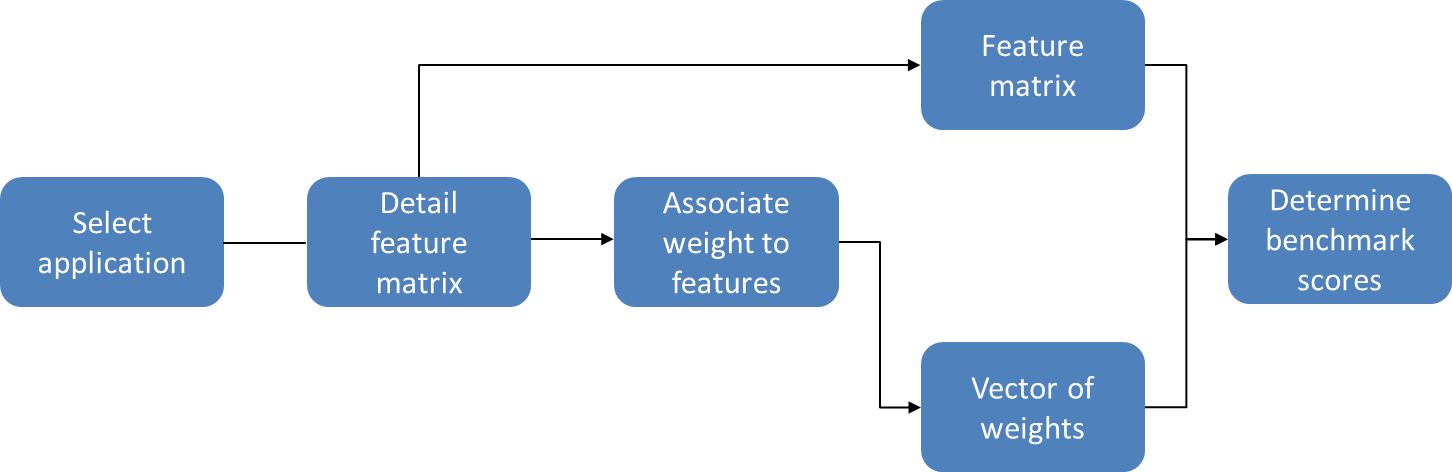
\includegraphics[width=0.9\textwidth]{images/benchmark_process}
\caption{Benchmarking process}
\label{fig:bench_process}
\end{figure}
In this section I will describe a formal model that will allow us to determine a benchmark score for a given application and a given sensor technology. As previously explained the different applications are distinguished by applying a different set of weights to the known features. As a start the process of this feature weighting is discussed and some examples about proper application are given. Afterwards, the formal model is introduced that deduces a single score benchmark for any sensor technology and any application. The overall process is shown in Figure \ref{fig:bench_process} and will be detailed in the following sections, including some example calculations.
\subsection{Feature score and weighting}
\label{ch:bench_sec_featscore}
The presented feature matrix has some ratings that need detailing in order to be quantifiable in the specific application. The ordinal measurements of the feature matrix should be assigned a quantifiable measure. Taking “Unobtrusiveness” the open system can be detailed as “visible by users” and “large system” as size larger than 100 x 100 x 100 mm. Similar level of details can be applied to the other features leading to the application-specific detailed feature matrix that is used in the scoring process. The different ratings are assigned different numeric values, namely 0.00 (--), 0.25 (-), 0.5 (o), 0.75 (+) and 1.00 (++). The weight of the features for the specific application is also rated on a 5-point ordinal scale, denoted as “not important” (numeric value 0.0), “less important” (0.25), “moderately important” (0.5), “important” (0.75) and “very important” (1.00). Thus for each application there is a distinct detailed feature matrix and a vector of associated weights that can be applied to a set of sensor technologies in order to calculate the benchmark score. The next step is to formally introduce the model that allows to determine a benchmarking score from feature ratings and application weights.
\subsection{Modeling}
The model is supposed to formalize a benchmark for any application and any sensor technology in any domain. As a start the following definitions are given:
\begin{itemize}
\item Set of $n$ domains \(D=\{d_1,...,d_i,...,d_n\}\)
\item Set of $m$ applications \(A=\{a_1,...,a_j,...,a_m\}\)
\item Set of $o$ features \(F=\{f_1,...,f_k,...,f_o\}\)
\item Set of $p$ sensor technologies \(S=\{s_1,...,s_l,...,s_p\}\)
\end{itemize}
In any domain $d_i$ there is have a set of potential applications \(A_{d_{i}}\subseteq A\) and a set of relevant features \(F_{d_{i}}\subseteq F\). For each feature \(f_{k,d_{i}}\subseteq A\) there is the associated feature score \(r_{F_{d_i}}\) as explained in the previous section. Each sensor technology $s_l$ has a specific feature score \(r_{s_l,F_{d_i}}\) with normalization \(\left \| r_{s_l,F_{d_i}} \right \|\epsilon [0,1]\).
\begin{equation}
\overrightarrow{r_{s_l,F_{d_i}}}= \begin{pmatrix}
r_{s_l,f_{1,_i}}\\ 
\vdots\\
r_{s_l,f_{o,_i}}
\end{pmatrix}
\end{equation} 
The weights $w_{f_o}$ associated to a specific application $a_j$ in a domain $d_i$ have the same cardinality $\left | w \right |$ as the vector of feature scores $\left | \overrightarrow{r_{s_l,F_{d_i}}} \right |$. The values are determined, so \(\left \| w_{f_o} \right \|\epsilon [0,1]\).
\begin{equation}
\overrightarrow{w_{a_j}}=\begin{pmatrix}
w_{f_1,a_j}\\ 
\vdots\\
w_{f_o,a_j}
\end{pmatrix}
\end{equation}
The feature scores and associated weights allows to determine a benchmark score $b_{s_l}$ for a specific sensor technology $s_l$ for any application $a_j$ by using the scalar product of feature score and respective weight and apply normalization with regard to the weight.
\begin{equation}
b_{s_l}=\tfrac{\overrightarrow{r_{s_l,F_{d_i}}}\cdot \overrightarrow{w_{a_j}}}{\sum_{k=1}^{o}w_{f_k,a_j}}
\end{equation}
Thus it is possible to compare different sensor technologies by calculating and comparing the different benchmark scores for a given set of sensor technologies $S_p\subseteq S$ and receive a set $B_{S_p}$ with $t=\left | s_p\right |$.
\begin{equation}
B_{S_p}=\{b_{s_l,1},\hdots,b_{s_l,t}\}
\end{equation}
In order to determine the optimal (chosen) sensor technology $b_c$ for an application $a_j$ and given the prerequisites regarding non-negativity of weights and feature scores we can evaluate the set for the maximum element.
\begin{equation}
b_c=max(B_{S_p})
\end{equation}
\subsection{Feature score normalization}
With regards to actual benchmarking the problem of bias towards a specific technology may occur. If the average features ratings are different between two technologies the calculated benchmark score will increase. In many instances this might be beneficial, yet if comparing numerous technologies to a set of different applications a trend might be more important than absolute scores. Thus, we provide an optional step of calculating the normalized feature vector $r_{s_l,F_{d_i},norm}$ with regard to the average associated value of $0.5$, using the following equation.
\begin{equation}
\overrightarrow{r_{s_l,F_{d_i},norm}}= \begin{pmatrix}
r_{s_l,f_{1,_i}}\\ 
\vdots\\
r_{s_l,f_{o,_i}}
\end{pmatrix}
\cdot \tfrac{o\cdot0.5}{\sum_{p=1}^{o}r_{s_l,f_{p,d_i}}}
\end{equation} 
The feature-normalized benchmark score is accordingly determined with the following equation.
\begin{equation}
b_{s_l}=\tfrac{\overrightarrow{r_{s_l,F_{d_i},norm}}\cdot \overrightarrow{w_{a_j}}}{\sum_{k=1}^{o}w_{f_k,a_j}}
\end{equation}
\subsection{Scoring}
Now with the formal model and the available set of feature matrix and weights we are able to calculate the benchmarking score for a set of sensor technologies. As an example we are choosing the application indoor localization in a public shopping area to monitor customer behavior. The requirements include a tracking accuracy of 50 cm, with a large area to cover and potentially fast moving persons. Thus the importance ratings for performance characteristics are moderately important for resolution, important for update rate and very important for detection range. The system can also be used for security purposes, thus unobtrusiveness is less important. There can be dedicated servers, so processing complexity is not important, but the system should be difficult to disturb, thus robustness is important. Disturbance frequency is moderately important, as a large number of per-sons is monitored, leading to statistically significant results, even if single measurements are disturbed. The environment is fairly static, thus calibration complexity is less important. It is possible that a crowded shop produces a lot of acoustic noise, therefore no unique limitations towards acoustic disturbances should be present and this is moderately important. The resulting vector of weights is:
\begin{equation}
\overrightarrow{w_a}=
\begin{pmatrix}
0.50 & 0.75 & 1.00 & 0.25 & 0.00 & 0.75 & 0.50 & 0.25 & 0.50
\end{pmatrix}^{-1}
\end{equation}
Based on previous experiences and best practice a camera-based system is evaluated. The system has high resolution cameras, with an update rate of 30 samples per second and a high detection range of more than 20 meters. The cameras are external, not hidden from view but attached on the ceiling. The processing complexity is very high, requiring a dedicated system per camera. Since they are out of reach they are robust towards human intervention and independent from each other. In the given setting visual disturbance is unlikely, calibration is difficult but not required regularly and the system is not disturbed by acoustic noise. This results in the following rating vector:
\begin{equation}
\overrightarrow{r_{s,f}}=
\begin{pmatrix}
1.00 & 0.75 & 1.00 & 0.25 & 0.00 & 0.50 & 0.75 & 0.25 & 1.00
\end{pmatrix}^{-1}
\end{equation}
Using those two vectors we can calculate the final scoring for this sensor system using the equations of the previous section, leading to $b_s \approx 0.78$ and a feature-normalized score of $b_{s,norm} \approx 0.63$. Determining the feature rating vector for other technologies is possible in a similar fashion. The optimal technology would have the highest score $b_s$ or $b_{s,norm}$.
\clearpage
\section{Evaluating technology popularity}
In order to evaluate the method we propose a discussion based on previous successful works in the domain of smart environments. We will select three different application areas and for each benchmark three different sensor technologies. In order to estimate how popular a certain technology is for a given application we will be using the ACM Digital Library to query scientific publications with respective author keywords. This method is limited, as the chosen keywords may not catch all relevant publications. Therefor we will slightly increase the focus by using multiple associated search terms for each application and technology. Additionally we will also perform respective searches using the Google Scholar data-base that has a much broader scope-The advantages of the latter are the huge collection of scientific resources and no strong selection bias. However, there are various associated issues that may affect the method. The search results vary on the search term, additionally there will be results that mention the search term but do not necessarily rely on the technology for their respective system. Therefore, the results should be considered as an indicator for popularity in the research community. Similar to the ACM DL search we are also looking for synonyms and calculate an average between the search results.

As applications we choose hand gesture interaction, a marker-based identification system and obstacle avoidance for an autonomous system. The technologies are camera systems, radio-based systems, depth or stereo cameras and ultrasound devices.
\subsection{Scoring}
% Table generated by Excel2LaTeX from sheet 'Tabelle1'
\begin{table}[htbp]
  \centering
  \caption{The importance weighting of different applications, based on the features.}
    \begin{tabular}{rrrrrrrrrr}
    \toprule
          & res   & upd   & det   & unob  & proc  & robu  & disfr & calco & uniqd \\
    \midrule
    Hand Gesture & ++    & ++    & -     & -     & -     & o     & +     & o     & o \\
    Identification & --    & -     & ++    & ++    & o     & ++    & +     & -     & + \\
    Obstacle Avoidance & -     & +     & -     & o     & +     & +     & ++    & ++    & + \\
    \bottomrule
    \end{tabular}%
  \label{tab:bench_appweights}%
\end{table}%
At first we determine the weights of the different applications with regards to the features. The results are shown in Table \ref{tab:bench_appweights}. For the tables in this section we are using short notation of the features in order of appearance in Section \ref{ch:bench_sec_featscore}.
\begin{table}[htbp]
  \centering
  \caption{Feature rating of the different sensor technologies}
    \begin{tabular}{rrrrrrrrrr}
    \toprule
          & res   & upd   & det   & unob  & proc  & robu  & disfr & calco & uniqd \\
    \midrule
    Camera & ++    & o     & +     & -     & o     & o     & o     & -     & o \\
    Radio & -     & +     & ++    & +     & o     & o     & o     & o     & - \\
    Depth camera & +     & o     & o     & -     & -     & o     & -     & o     & o \\
    Ultrasound & -     & +     & o     & o     & +     & o     & +     & o     & o \\
    \bottomrule
    \end{tabular}
  \label{tab:bench_feature_rating}
\end{table}
The rating of the different technologies and the resulting score is shown in Table \ref{tab:bench_feature_rating}. Here it is possible to follow different strategies regarding the rating. In terms of unbiased comparison looking at the equations it would be necessary that all technologies have the same average feature rating. The second strategy is to apply an absolute ranking to all technologies, independent of the given application. This might lead to certain technologies being unsuited for a given task, or technologies that have the best benchmark score regardless of application. In this specific case the average rating is 0.53 for cameras, 0.58 for radio, 0.44 for depth cameras and 0.56 for ultrasound devices. Table \ref{tab:bench_scores} displays the different calculated benchmark scores for the combinations between applications and technologies. As we are comparing numerous technologies and applications the feature-normalized benchmark score is also included.

\begin{table}[htbp]
  \centering
  \caption{Regular and normalized benchmark score matrix of different applications and technologies}
    \begin{tabular}{rrrrrr}
    \toprule
          &       & Camera & Radio & Depth Camera & Ultrasound \\
    \midrule
    \multirow{2}[0]{*}{Hand Gesture} & $b_{s_l}$ & 0.58  & 0.53  & 0.49  & 0.55 \\
          & $b_{s_l,norm}$ & 0.54  & 0.45  & 0.55  & 0.50 \\
          \midrule
    \multirow{2}[0]{*}{Identification} & $b_{s_l}$ & 0.49  & 0.64  & 0.40  & 0.57 \\
          & $b_{s_l,norm}$ & 0.46  & 0.55  & 0.45  & 0.51 \\
          \midrule
    \multirow{2}[0]{*}{Obstacle Avoidance} & $b_{s_l}$ & 0.47  & 0.56  & 0.42  & 0.59 \\
          & $b_{s_l,norm}$ & 0.44  & 0.48  & 0.47  & 0.53 \\
    \bottomrule
    \end{tabular}%
  \label{tab:bench_scores}%
\end{table}%
The effect of the normalization is easily visible. Particularly radio has a high feature rating and is negatively affected by the normalization. The only example with a negative average feature rating is the depth camera. After applying the normalization it becomes competitive in some applications.

Finally, Table \ref{tab:bench_search_res} shows the search results regarding the different technologies and applications. Particularly the ACM DL keyword search can generate empty results if the search terms are too specific. Thus, the search terms we were using are “gesture“, “identification and “obstacle” in this regard and add synonyms for the different technologies. For each sensor category we allowed the following synonyms. “Camera” and “video” for the first technology, “radio”, “rf” and “wifi” for the second, “depth camera”, “stereo camera” and “Kinect” for the third and “ultrasound” as well as “ultrasonic” for the last one. All search results were averaged according to the number of synonyms used For the Google Scholar search we used more specific terms, “hand gesture”, “user identification” and “obstacle avoidance” with the same synonyms to prevent an excessive number of search results and prevented inclusion of patents and citations. All searches were performed on January 30th, 2014.
% Table generated by Excel2LaTeX from sheet 'Tabelle1'
\begin{table}[htbp]
  \centering
  \caption{Search result frequency given specific applications, sensor technologies and synonyms for ACM Digital Library (DL) and Google Scholar (GS)}
    \begin{tabular}{rrrrrrrrrr}
    \toprule
          & \multicolumn{2}{r}{Camera} & \multicolumn{2}{r}{Radio} & \multicolumn{2}{r}{Depth Camera} & \multicolumn{3}{r}{Ultrasound} \\
    \midrule
          & DL    & GS    & DL    & GS    & DL    & \multicolumn{2}{r}{GS} & DL    & GS \\
    Hand Gesture & 66    & 14100 & 27    & 7350  & 32    & \multicolumn{2}{r}{6850} & 3     & 1660 \\
    Identification & 81    & 5590  & 162   & 4920  & 10    & \multicolumn{2}{r}{3957} & 5     & 599 \\
    Obstacle Avoidance & 8     & 24000 & 1     & 13017 & 17    & \multicolumn{2}{r}{12278} & 8     & 14500 \\
    \bottomrule
    \end{tabular}%
  \label{tab:bench_search_res}%
\end{table}%

\section{Discussion}
In this evaluation we included both benchmark score types to outline their dif-ferences. “Camera”, “radio” and “ultrasound” have a feature rating above average, whereas “depth cameras” had a lower than average rating. The feature-normalized benchmark score is thus adapted accordingly. Regarding the application of “hand-gesture recognition” this leads to “depth cameras” being considered the optimal technology as opposed to “cameras” that had a higher score before normalization. For the other applications there is no change in optimal technology. The preferred strategy for applying feature-normalized or non-feature-normalized benchmark scoring should depend on the specific benchmarking process. If we are bench-marking numerous technologies and applications in a single process the feature-normalization might be helpful to get a tendency regarding the optimal system. However, if the application is very specific it might be preferred to get a clear ranking and penalize unsuited technologies, regardless of their average feature weight. Accordingly, it is possible to refrain from normalization.
Looking at the search results we can draw several conclusions. The prevalence is unequally distributed between the different technologies. Both in keywords and general occurrence cameras are the most commonly occurring sensor device, with radio and depth camera ranked behind. Ultrasound on the other hand is less frequently occurring. This may be explained by the higher versatility of the other options. Regarding the “hand gesture” application, cameras have both the highest benchmark scores and most results in the database searches. The benchmark score for “user identification” and “radio” are matched for the ACM DL. However, there are more GS results for “camera”. As already mentioned cameras are more com-monly used, yet, the difference in keyword search results is significant. “Obstacle avoidance” is least common in the ACM DL, however quite popular in GS. Accordingly, “ultrasound” sensors are significantly more common in both searches, as opposed to the previous applications. Nonetheless, “stereo cameras” are the most common sensor device for this application. They are commonly used in automotive scenarios, where the detection range of ultrasound is insufficient, as the objects are moving fast \cite{bertozzi1998gold}. Therefore, the application scenario might have to be redefined for fast-moving object detection in open areas as opposed to obstacle avoidance for robots in home scenarios. 
We additionally have to discuss the method of using database searches for verifying the benchmarking method, as opposed to expert opinion. Surveys of a specific application or certain technologies are common in scientific literature. How-ever, while they might be comprehensive and cite several hundred different applications, the ACM DL database covers more than 2.2 million entries and GS searches can lead to more than 9.7 million results. Therefore, the index searches are preferable in terms of broadness. The search for keywords in ACM DL results in few hits compared to the database size. As they are chosen by the authors there is a large variety in word choice, spelling or number of keywords. While extend-ing the number of different searches might lead to more results overall, it may also lead to additional overshoot, including work that do not cover the desired topics. The GS searches are very prone to overshooting, and should be preferably used to discover trends in data, as opposed to narrowly clustered results.
Finally we want to briefly discuss the tendency of the benchmark scores to crowd around 0.5. While the benchmark may result in any number between 0 and 1 the two normalization processes and the tendency to avoid extreme scoring for features and weights leads to an average close to 0.5. Thus, even slower differences close to this average may have a higher significance. It would also be possible to put more emphasis by using a correction term.

\section{Applications for capacitive proximity sensors}
